To begin implementing lighting, we must first establish a light source in the form of a directional light. Directional light sources uniformly light objects in the scene from one direction, similar to how the sun illuminates objects on Earth. We can define a directional light using two parameters:
$$ \hat{L} \text{ a \textbf{normalized} three dimensional vector representing the direction of the light}$$
$$ \Vec{I} \text{ a three dimensional color vector representing the intensity of the light}$$
For shading, we will use a modified Phong shading model only including the ambient and diffuse lighting components:
$$
\text{Color} = \Vec{K}a + \sum_{n \in \text{lights}}(\Vec{K}\Vec{I}_{n}(\hat{L}_{n} \cdot \hat{N}))
$$
Where $\Vec{K}$ is three dimensional vector representing the color of the object, $a$ is the ambient lighting coefficient ($0 \leq a < 1$), $\hat{L}_n$ is the direction of light $n$, $I_n$ is the intensity of light $n$, and $\hat{N}$ is the surface normal of the object. Note that the multiplication of $\Vec{K}$ and $\Vec{I}_n$ is a component-wise product. To better understand what this equation is doing, we can break it up into parts, beginning with the ambient component.
$$\Vec{K}a$$
In the real world, objects usually receive some indirect lighting from their surroundings even when they are in shadow or when there is no direct light source present. The ambient component accounts for this by allowing for slight illumination of unlit surfaces. Since $a$, the ambient lighting coefficient, is always less than 1, ambient lighting will naturally be less than lighting from direct light sources, ensuring that unlit areas will appear darker than areas in direct light. Next, we can take a look at the diffuse lighting component.
$$\Vec{K}\Vec{I}_{n}((-\hat{L}_{n}) \cdot \hat{N})$$
Diffuse shading aims to model the appearance of rough, non-reflective surfaces like paper. The dot product between $-\hat{L}_{n}$ and $\hat{N}$, both normalized vectors, essentially acts as a measure of similarity of the light direction and surface normal. If the surface normal and light direction are pointing directly towards each other (light is pointing towards the surface), this value will be 1, 0 if perpendicular, and -1 if pointing in the same direction (light is pointing away from the surface). This is very useful for lighting calculations as we only want to illuminate surfaces that are facing the light source. Therefore, if the result of the dot product is less than 0, we know that the surface should receive no light from light source $n$. If the result is greater than zero, we scale the intensity of light source $n$, $\Vec{I}_n$, by the result. Finally, we perform a component-wise multiplication of $\Vec{K}$ and $\Vec{I_n}$ to obtain our final diffuse lighting component. Note that in the full equation, this component is summed over all light sources in the scene and then added to the ambient component to get the final color for a specific pixel. Implementing lighting into our earlier scene configuration with a white sphere and a directional light pointing in the direction $\begin{bmatrix}-1, -1, 1\end{bmatrix}$ (Automatically normalized in the actual implementation) with a uniform intensity of $\begin{bmatrix}1, 1, 1\end{bmatrix}$ gives us the following image:
\begin{figure}[H]
    \centering
    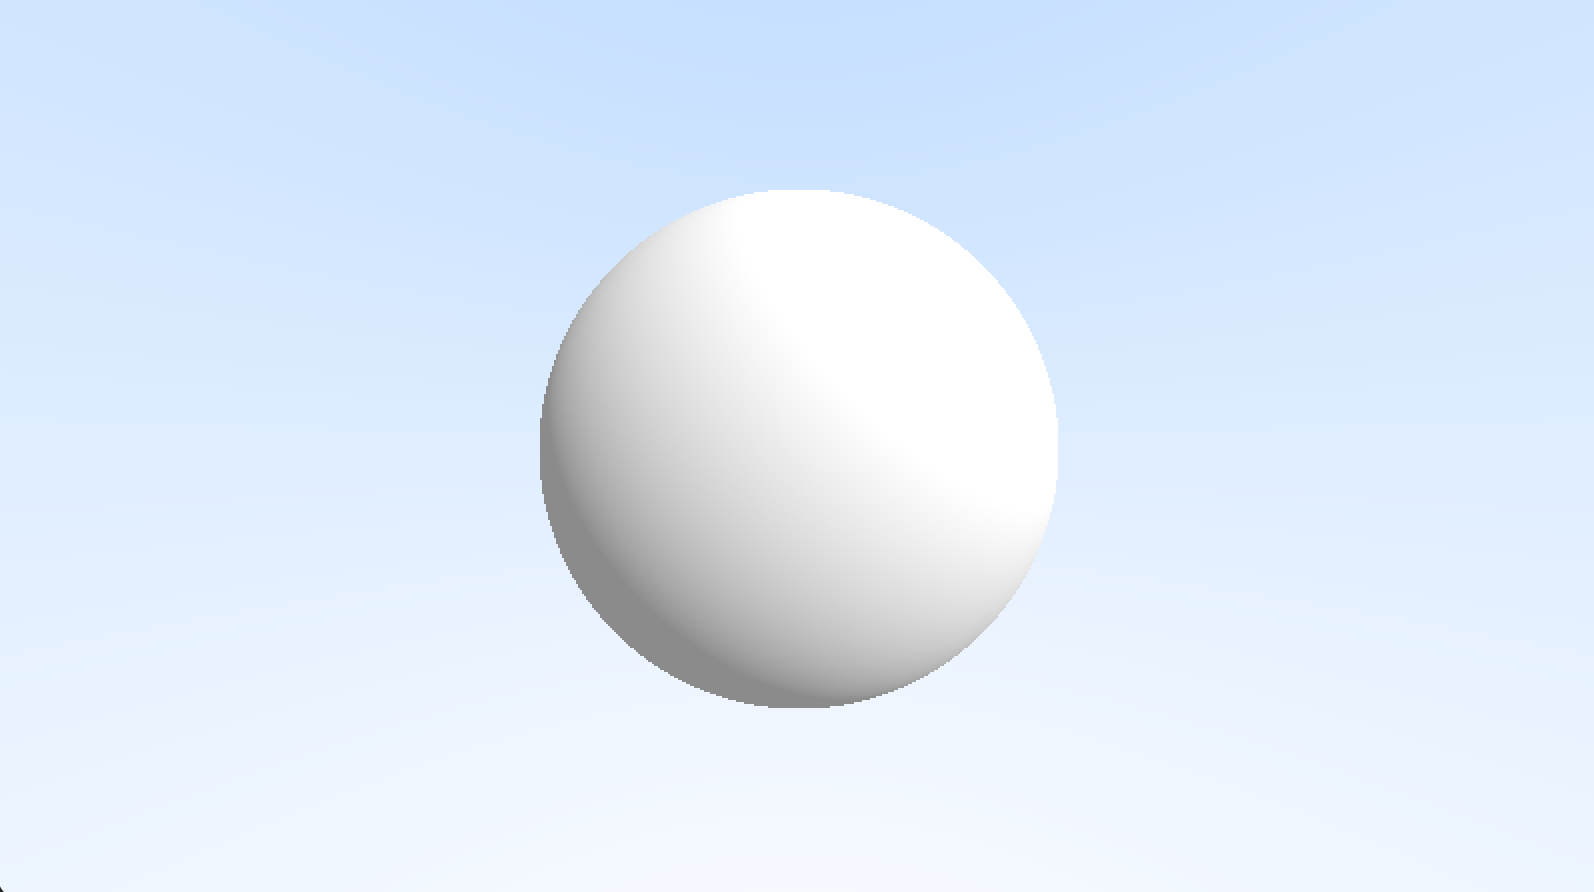
\includegraphics[scale=0.4]{figures/DiffuseSphere.png}
    \caption{Sphere with diffuse shading from a directional light}
    \label{fig:diffuse_sphere}
\end{figure}